\documentclass{article}
\usepackage{ctex}
\usepackage{amsmath}
\usepackage{graphicx}
\usepackage{subfigure}
\graphicspath{{figure/}}
\usepackage[section]{placeins}
\usepackage{float}
\usepackage{appendix}
\usepackage{amstext}
\usepackage{listings}
\lstset{language=Matlab}%语言
\title{可激发系统的模拟:Hodgkin-Huxley神经元模拟}
\date{2020.4.15}
\author{俞炀}

\begin{document}
	\maketitle
	\begin{abstract}
		Hodgkin-Huxley模型是1952年Hodgkin和Huxley利用Cole发明的电压钳位技术获得了乌贼轴突电生理活动的大量实验数据,并在这些数据的基础上推导出一个采用四维非线性微分方程系统描述的数学模型。该模型能够准确的解释实验结果,量化描述了神经元细胞膜上电压与电流的变化过程。本文第一部分为通过对HH模型参数赋值,根据四个微分方程,运用R—K四步法,求解出在不同电流刺激下动作电位随着时间得变化;第二部分为计算直流刺激强度和神经元发放频率之间的关系;最后,计算一个动作电势过程中通过单位面积细胞膜的钠离子总数目。	
		\textbf{关键词:}\qquad Hodgkin-Huxley模型  \qquad Runge-Kutta四步法 
	\end{abstract}
	
	\section{HH神经系统模型}
	\subsection{背景知识介绍}
	\begin{itemize}
		\item 神经元所传导的信号是电信号,当神经元在静息,即没有外界扰动的时候,其细胞膜膜内和膜外存在一电势差(约为-70mV),我们称之为膜电势;当其受到外界扰动(在实验中以一个电流扰动输入代替外界刺激),且超过系统阈值,则膜电势将产生一个较为陡峭的变化,产生动作电势(action potential),此时神经元处于被激发状态。通过控制输入电流的频率以及振幅,我们可编码外界信息。
		\item 神经元跨膜电势差产生的原因是:神经元细胞内外分布大量带点离子,如:Na离子,K离子等,且其浓度存在差异,与此同时,其膜内外还存在电场。在浓度梯度以及电场作用达到平衡的状态时,神经元细胞产生了静息时的跨膜电势差。其定量描述的数学表达主要为两个方程:
		\begin{align}%多行公式,每行公式后面标号,如想不标号,则添加\nonumber
		&\text{能斯特方程(单离子情形)}\nonumber\\%&为对齐符号,\text为插入文档,文档中插入特殊字符或者公式等(一般是特殊字符),用$$。\\为换行符号。
		& V_{K} = \frac{KT}{q}\ln\frac{[K]_{out}}{[K]_{in}}\\
		&\text{Golden-Hodgkin-Katz方程(多离子情形)}\nonumber\\
		&V_{m}=\frac{RT}{F}\ln(\frac{p_{K}[K^{+}]_{0}+p_{Na}[Na^{+}]_{0}+p_{Cl}[Cl^{+}]_{i}}{p_{K}[K^{+}]_{i}+p_{Na}[Na^{+}]_{i}+p_{Cl}[Cl^{+}]_{0}})
		\end{align}
		\item 离子通道是神经元在受到外界刺激时,产生动作电位原因。离子通道为蛋白质分子形成的离子的跨膜的管道,允许离子进行跨膜流动。其有如下性质:
		\begin{itemize}	
			\item[a] 开关性 
			通过感应膜内外电势差变化,离子通道进行打开或者关闭;或者离子通道与神经壁质相结合/脱离时通道开启/关闭
			\item[b] 选择性
			某种离子通道只允许特定离子通过。
		\end{itemize}
		\item 神经元等效电路模型极其公式:
		如图\ref{1},$C_{m}$为细胞膜的膜电容,后面三个支路分别代表对应的离子与其离子通道进行跨膜流动的路径。由等效电路,通过基尔霍夫定理,我们可以轻松得到其等效电流方程。
		\begin{figure}[H]
			\centering
			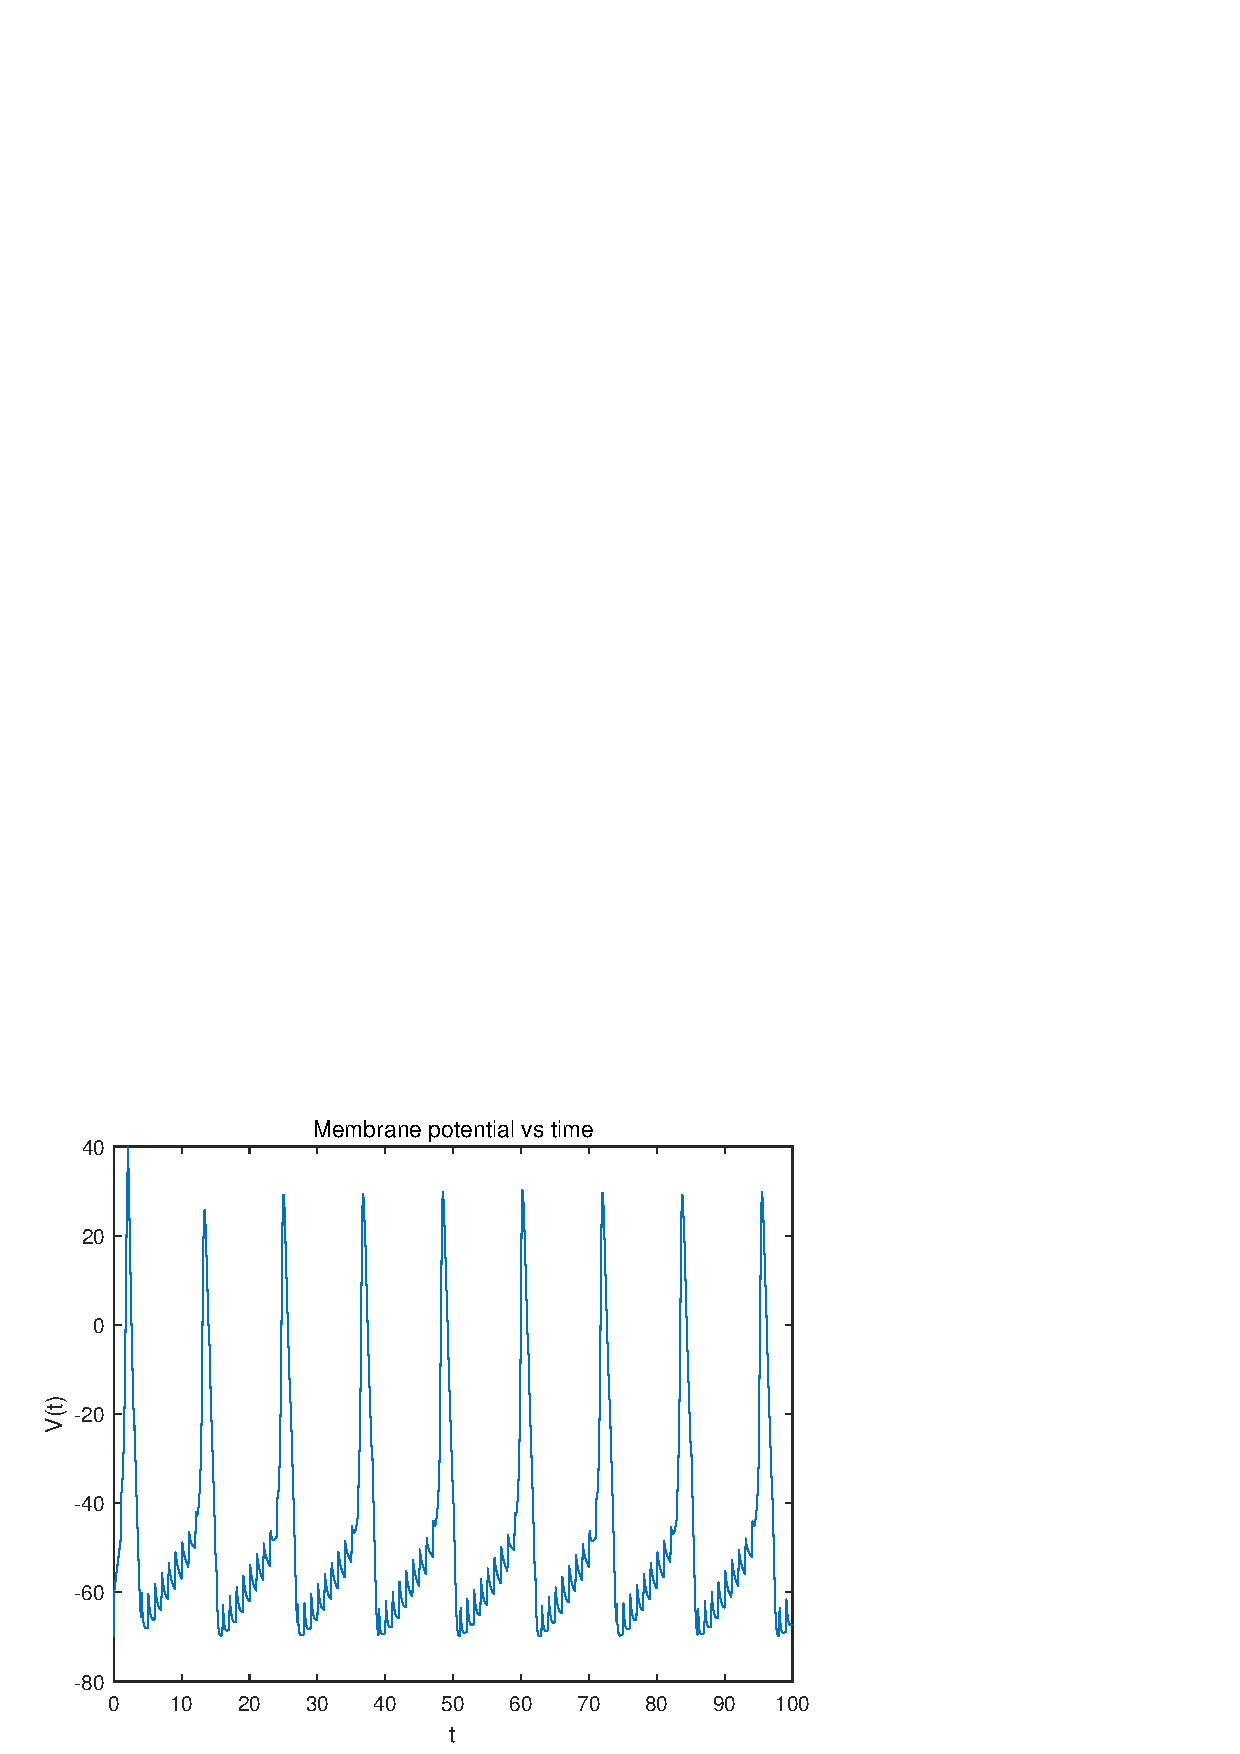
\includegraphics[scale=0.5]{1.png}
			\caption{神经元等效电路模型}\label{1}
		\end{figure}
	\end{itemize}

	\subsection{HH模型的数学公式及解释}
	HH模型的四个微分方程组:
	\begin{align}
	&C_{m}\frac{dV}{dt}=-g_{L}(V-E_{L})-\overline{g}_{Na}m^3h(V-E_{Na})-\overline{g}_{K}n^4(V-E_{K})+I_{app} \label{f1}	\\
	&\frac{dm}{dt}=\alpha_{m}(V)(1-m)-\beta_{m}(V)m\\
	&\frac{dh}{dt}=\alpha_{h}(V)(1-h)-\beta_{h}(V)h\\
	&\frac{dn}{dt}=\alpha_{n}(V)(1-n)-\beta_{n}(V)n
	\end{align}
	其中在公式\ref{f1}中,$g_L$,$\overline{g}_{Na}$,$\overline{g}_{K}$分别代表电路、Na离子、钾离子电导率;m,h,k为描述离子开关行为的变量,符合一阶常微分方程。
	
	
	\section{不同刺激强度下神经元膜电势变化}
	\subsection{刺激电流恒定的情况}
	当刺激电流$I_{app}=10$始终不发生变化时,神经元膜电势情况如下图\ref{t1}所示:
	\begin{figure}[H]
		\centering
		\includegraphics[scale=0.5]{t1}
		\caption{刺激电流恒定为10}\label{t1}
	\end{figure}
	
	\subsection{脉冲刺激}
	下图\ref{t1p}描述的是在脉冲刺激下的膜电位的变化情况,每间距一定时间,刺激电流$I_{app}$会从10增至100;其中下图\ref{t1p1},图\ref{t1p2},图\ref{t1p3},图\ref{t1p4},图\ref{t1p5},图\ref{t1p6}分别为间隔时间1s,5s,10s,20s,50s,80s下的膜电位变化情况。
	\begin{figure}[H]%H表示优先放置的图片位置
		\centering
		
		\subfigure[间距为1的脉冲]{
			\begin{minipage}[t]{0.4\linewidth}
				\centering
				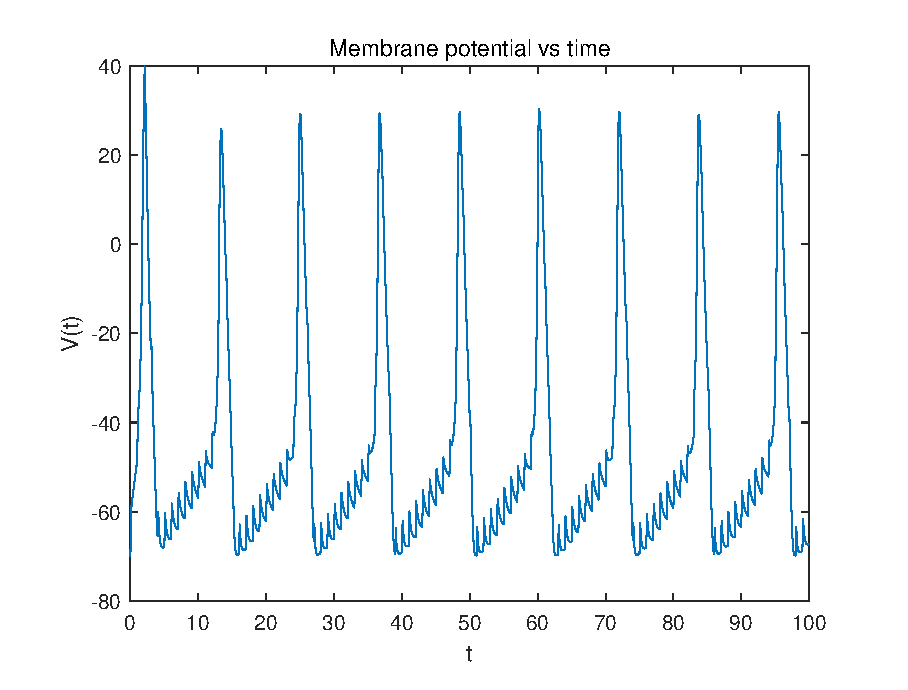
\includegraphics[width=2in]{1.eps}
				\label{t1p1}
				%\caption{fig1}
			\end{minipage}%
		}%
		\subfigure[间距为5的脉冲]{
			\begin{minipage}[t]{0.4\linewidth}
				\centering
				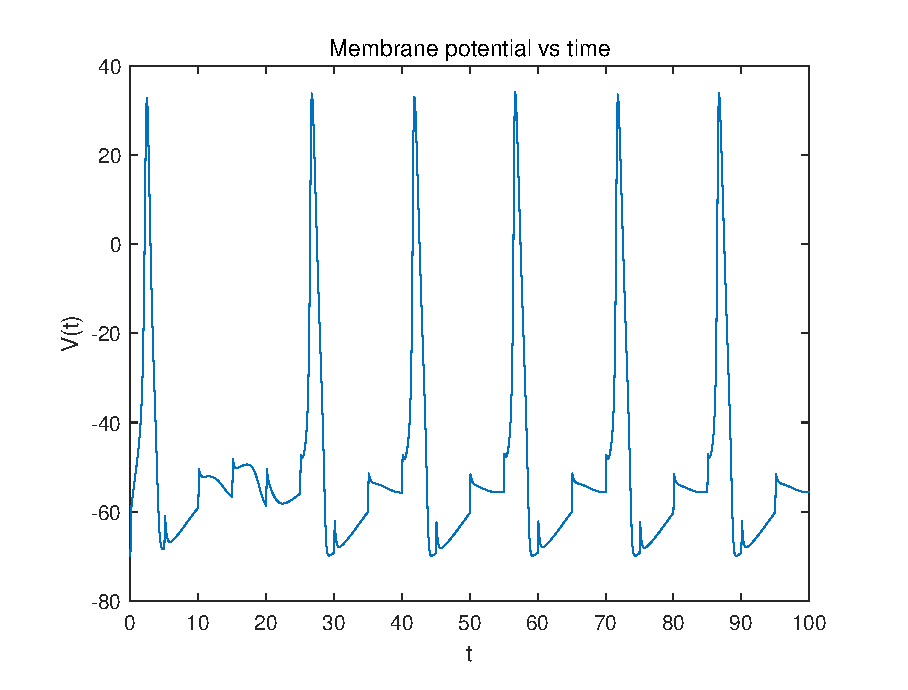
\includegraphics[width=2in]{5.eps}
				\label{t1p2}
				%\caption{fig2}
			\end{minipage}%
		}%	%这个回车键很重要 \quad也可以
		\quad
		\subfigure[间距为10的脉冲]{
			\begin{minipage}[t]{0.4\linewidth}
				\centering
				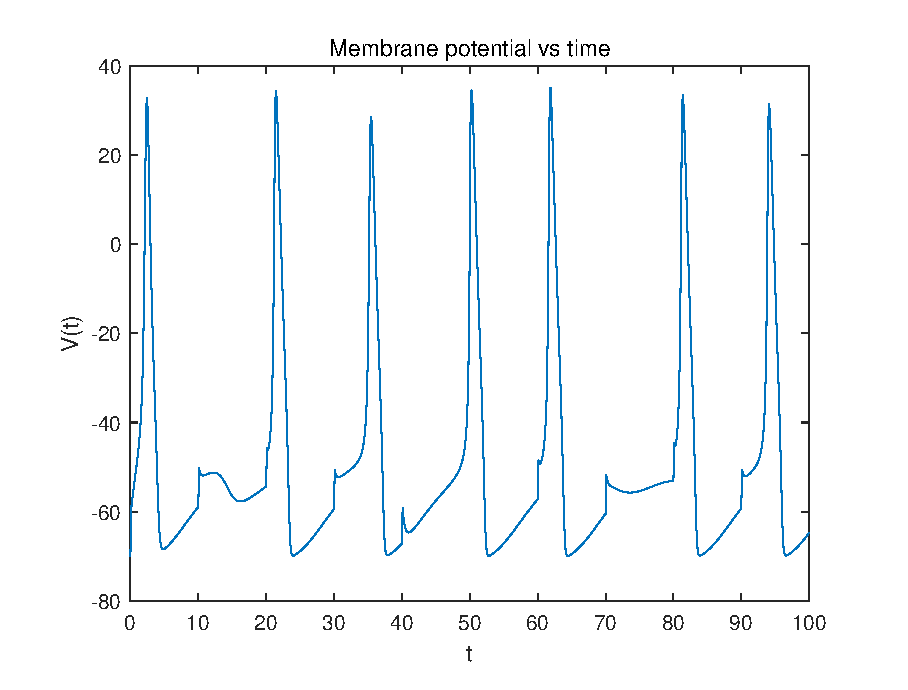
\includegraphics[width=2in]{10.eps}
				\label{t1p3}
				%\caption{fig2}
			\end{minipage}
		}%
		\subfigure[间距为20的脉冲]{
			\begin{minipage}[t]{0.4\linewidth}
				\centering
				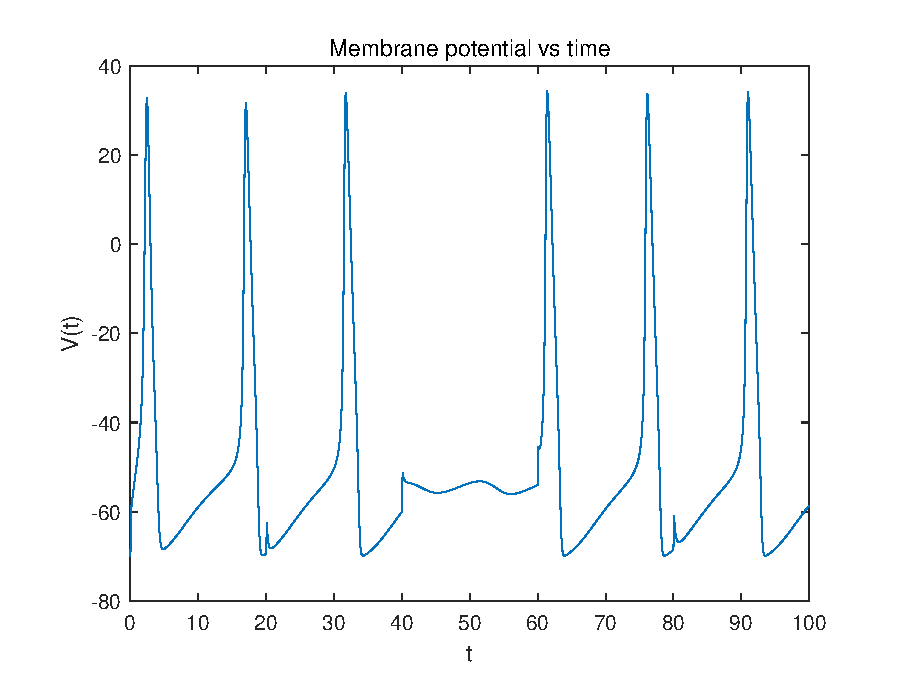
\includegraphics[width=2in]{20.eps}
				\label{t1p4}
				%\caption{fig2}
			\end{minipage}
		}%
		\quad	
		\subfigure[间距为50的脉冲]{
			\begin{minipage}[t]{0.4\linewidth}
				\centering
				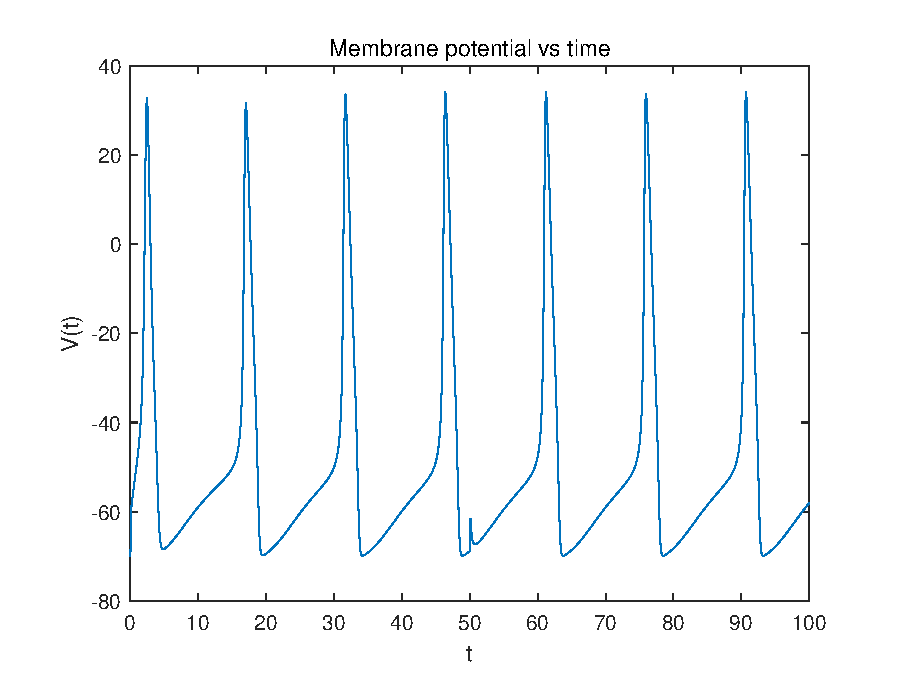
\includegraphics[width=2in]{50.eps}
				\label{t1p5}
				%\caption{fig2}
			\end{minipage}
		}%
		\subfigure[间距为80的脉冲]{
			\begin{minipage}[t]{0.4\linewidth}
				\centering
				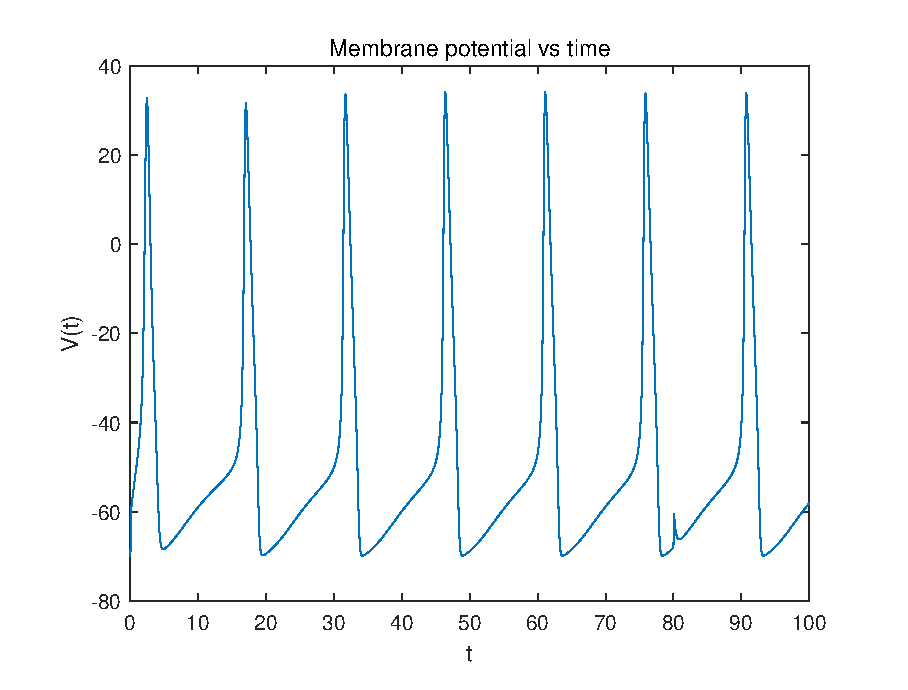
\includegraphics[width=2in]{80.eps}
				\label{t1p6}
				%\caption{fig2}
			\end{minipage}
		}%
		\centering
		\caption{不同时间间隔下的脉冲刺激所对应的动作电位}
		\label{t1p}
	\end{figure}
	\subsection{直流刺激}
	对神经元输入如图\ref{t1d1}的直流刺激信号,得到了神经元膜电势的变化情况如图\ref{t1d2}。由图\ref{t1d2}可知,随着电流强度的增大,其频率发生了显著的变化。
	\begin{figure}[H]%H表示优先放置的图片位置
		\centering
		
		\subfigure[脉冲电流I随时间t的变化]{
			\begin{minipage}[t]{0.4\linewidth}
				\centering
				\includegraphics[width=2in]{t1d1.eps}
				\label{t1d1}
				%\caption{fig1}
			\end{minipage}%
		}%
		\subfigure[t=1000,间隔100s的直流刺激下神经元膜电势随时间的变化]{
			\begin{minipage}[t]{0.4\linewidth}
				\centering
				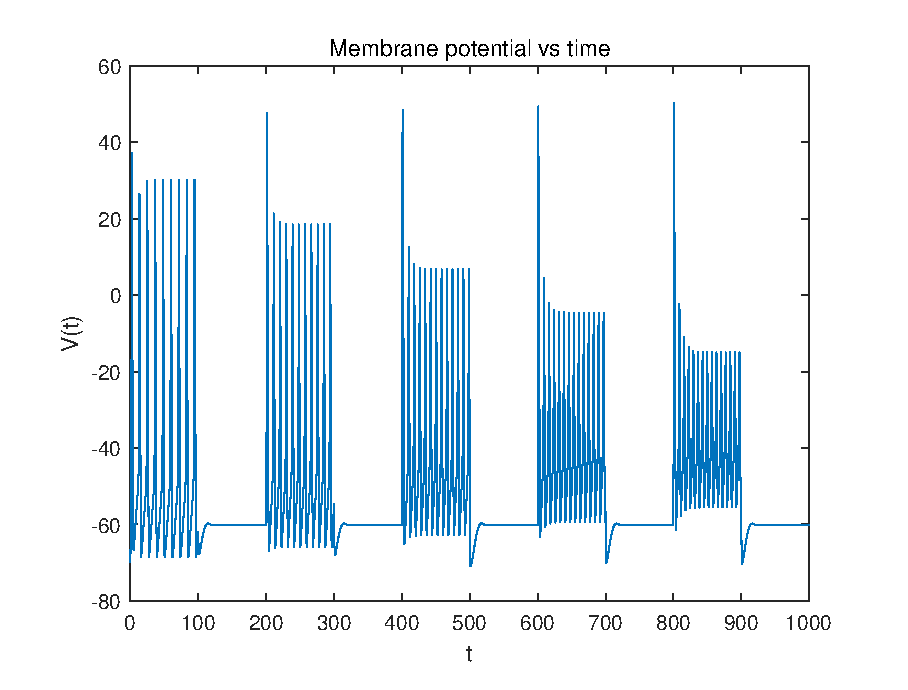
\includegraphics[width=2in]{t1d2.eps}
				\label{t1d2}
				%\caption{fig2}
			\end{minipage}%
		}
		\centering
		\caption{直流刺激}
		\label{t1d}
	\end{figure}
	
	\section{直流刺激下神经元动作电势频率随电流的变化}
	由图\ref{t1d2}可知,不同刺激电流下,动作电位的频率会发生显著变化。此处为探究周期/频率随时间的变化,取电位V大小为-40V为参照,遍历所有的V(i)。当且仅当V(i)>-40V,V(i+1)<-40V时,周期count+1。经探究发现,在I极小时(I<7),仅会出现一个起伏不大的峰,此后并无明显的动作电位的周期性产生,因此作者认定此不属于周期性变化的范围内,因而计数减一。经过修改调试,最终做得刺激电流与频率之间的关系如下:
	\begin{figure}[H]
		\centering
		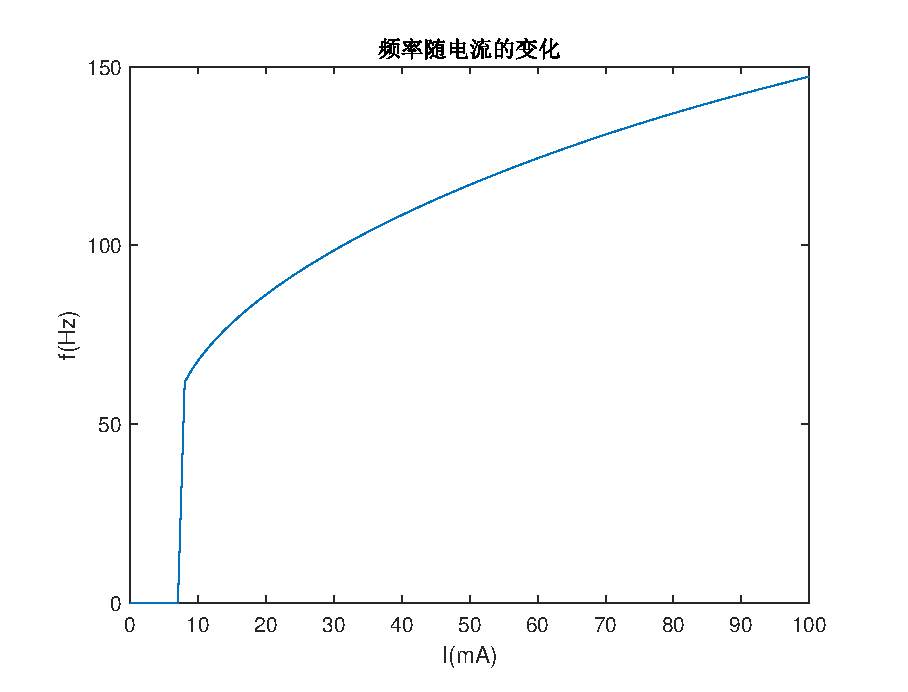
\includegraphics[scale=0.5]{t2}
		\caption{神经元动作电位频率随着刺激电流大小的变化}\label{t2}
	\end{figure}
	
	
	\section{一个动作电势过程中通过单位面积细胞膜的钠离子总数}
	由方程\ref{f1}可得所有的离散情况下的V(i)。根据公式$I_{Na} =-\overline{g}_{Na}m^3h(V-E_{Na}) $,$I_{K}\overline{g}_{K}n^4(V-E_{K}$,$I_{Cl}=-g_{L}(V-E_{L})$,可知三种离子电流分别随时间的变化。又因为$dQ = Idt$,积分可得流过的钠离子总电量,再通过总电量Q除以单位电荷,即可得一个动作电势过程中通过单位面积的钠离子总数。图\ref{t3}上方为钠离子,钾离子,氯离子电流随时间的变化,下方为钠离子流出电量随时间的变化。经计算可得,流出的钠离子总电量为:535.7498C,总粒子数为:$3.3484\times10^{21}$。
	\begin{figure}[H]
		\centering
		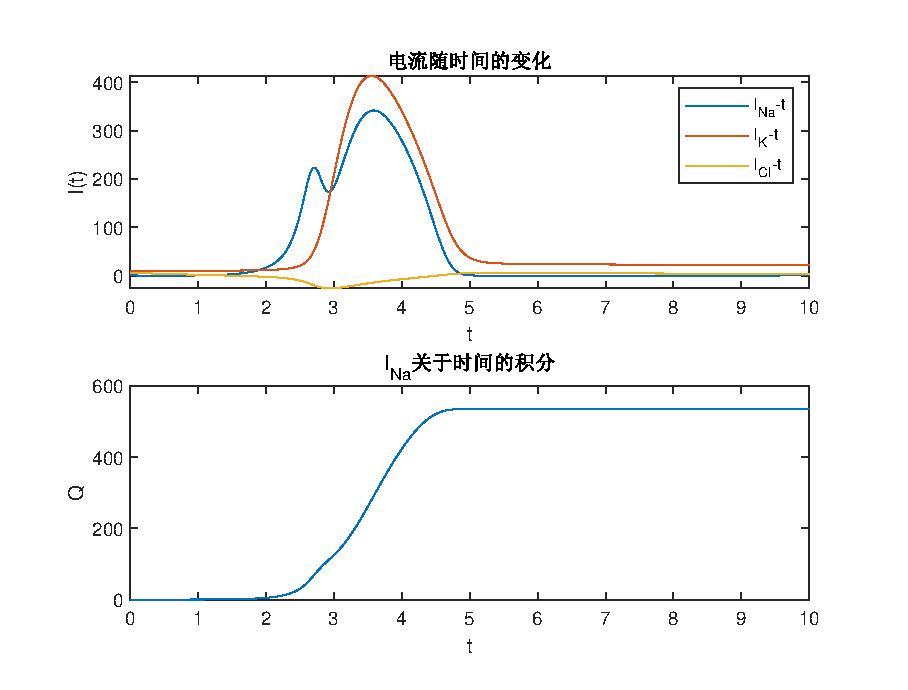
\includegraphics[scale=0.5]{t3}
		\caption{钠离子电流随时间的变化及其积分(钠离子流出电量随时间的变化)}\label{t3}
	\end{figure}
	
	
	%标序号粉分条叙述
%	\begin{itemize}	
%		\item[a]%序号a
%		\item[b]
%		\item[c]
%	\end{itemize}
	
	
	%画图(小图)
%	\begin{figure}[H]%H表示优先放置的图片位置
%		\centering
		
%		\subfigure[小图标题]{
%			\begin{minipage}[t]{0.4\linewidth}
%				\centering
%				\includegraphics[width=2in]{图片文件的名称}
%				\label{图片标签(引用的时候运用)}
%				%\caption{fig1}
%			\end{minipage}%
%		}%
%		\subfigure[小图标题]{
%			\begin{minipage}[t]{0.4\linewidth}
%				\centering
%				\label{图片标签(引用的时候运用)}
%				%\caption{fig2}
%			\end{minipage}%
%		}%	%这个回车键很重要 \quad也可以
%		\quad
%		\subfigure[小图标题]{
%			\begin{minipage}[t]{0.4\linewidth}
%				\centering
%				\includegraphics[width=2in]{图片文件的名称}
%				\label{图片标签(引用的时候运用)}
%				%\caption{fig2}
%			\end{minipage}
%		}%
%		\subfigure[小图标题]{
%			\begin{minipage}[t]{0.4\linewidth}
%				\centering
%				\includegraphics[width=2in]{图片文件的名称}
%				\label{图片标签(引用的时候运用)}
%				%\caption{fig2}
%			\end{minipage}
%		}%
%		\quad	
%		\subfigure[小图标题]{
%			\begin{minipage}[t]{0.4\linewidth}
%				\centering
%				\includegraphics[width=2in]{图片文件的名称}
%				\label{图片标签(引用的时候运用)}
%				%\caption{fig2}
%			\end{minipage}
%		}%
%		\subfigure[小图标题]{
%			\begin{minipage}[t]{0.4\linewidth}
%				\centering
%				\includegraphics[width=2in]{图片文件的名称}
%				\label{图片标签(引用的时候运用)}
%				%\caption{fig2}
%			\end{minipage}
%		}%
%		\centering
%		\caption{组图标题}
%		\label{总的组图标签}
%	\end{figure}
	
	%大图
%	\begin{figure}[H]
%		\centering
%		\includegraphics[scale=0.5]{图片文件名称}
%		\caption{图片标题}\label{图片标签}
%	\end{figure}
	
	
	%公式
%	\begin{align}%多行公式,每行公式后面标号,如想不标号,则添加\nonumber
%	&\text{$$}\nonumber\\%&为对齐符号,\text为插入文档,文档中插入特殊字符或者公式等(一般是特殊字符),用$$。\\为换行符号。
%	& \\
%	&\\
%	&\\
%	&\\
%	&\\
%	&\\
%	&\\
%	&\\
%	&\\
%	&
%	\end{align}
	
%	\begin{equation}%多行公式,尾部只有一个标号(一般不习惯在这里使用多行,基本当作单行公式使用)
	
%	\end{equation}
	
	
	
	\begin{appendix}	
		\section{不同刺激强度下神经元膜电势变化}
		\subsection{刺激电流恒定的情况}
\begin{lstlisting}	
clear all;clc;
global gK gNa gL VK VNa VL I C V_Na
gNa = 120; gK = 36; gL = 0.3;
VNa = 55; VK = -72; VL = -50;
C = 1; 
I = 10;
am = @(V) -0.1.*(35+V)./(exp(-0.1.*(35+V))-1);
bm = @(V) 4.*exp(-(60+V)./18);
		
ah = @(V) 0.07.*exp(-(60+V)./20);
bh = @(V) 1./(exp(-(30+V)./10)+1);
		
an = @(V) 0.01.*(-(50+V))./(exp(-0.1.*(50+V))-1);
bn = @(V) 0.125.*exp(-(60+V)./80);
		
fu = @(V,h,m,n,t) (-gL.*(V-VL)-gNa.*m.^3.*h.*(V-VNa)...
-gK.*n.^4.*(V-VK)+I)./C;
fm = @(V,h,m,n,t) am(V).*(1-m)-bm(V).*m;
fh = @(V,h,m,n,t) ah(V).*(1-h)-bh(V).*h;
fn = @(V,h,m,n,t) an(V).*(1-n)-bn(V).*n;
		
V(1)=-70;%电压初始值
n(1) = 0.1;m(1) = 0.1;h(1) = 0.1;%h,m,n初始值
t = linspace(0,100,10001);%时间间隔取为0-10秒之间的10000段
s = length(t);%t格点数
l = t(2)-t(1);%两时间点之间的时间间距
%四阶荣根库塔算法
		
		
for i = 1:1:s-1
k(1,1) = l.*fh(V(i),h(i),m(i),n(i),t(i));
k(2,1) = l.*fm(V(i),h(i),m(i),n(i),t(i));
k(3,1) = l.*fn(V(i),h(i),m(i),n(i),t(i));
k(4,1) = l.*fu(V(i),h(i),m(i),n(i),t(i));
k(1,2) = l.*fh(V(i)+1/2.*k(4,1),h(i)+1/2.*k(1,1),...
m(i)+1/2.*k(2,1),n(i)+1/2.*k(3,1),t(i)+l);
k(2,2) = l.*fm(V(i)+1/2.*k(4,1),h(i)+1/2.*k(1,1),...
m(i)+1/2.*k(2,1),n(i)+1/2.*k(3,1),t(i)+l);
k(3,2) = l.*fn(V(i)+1/2.*k(4,1),h(i)+1/2.*k(1,1),...
m(i)+1/2.*k(2,1),n(i)+1/2.*k(3,1),t(i)+l);
k(4,2) = l.*fu(V(i)+1/2.*k(4,1),h(i)+1/2.*k(1,1),...
m(i)+1/2.*k(2,1),n(i)+1/2.*k(3,1),t(i)+l);
k(1,3) = l.*fh(V(i)+1/2.*k(4,2),h(i)+1/2.*k(1,2),...
m(i)+1/2.*k(2,2),n(i)+1/2.*k(3,2),t(i)+l/2);
k(2,3) = l.*fm(V(i)+1/2.*k(4,2),h(i)+1/2.*k(1,2),...
m(i)+1/2.*k(2,2),n(i)+1/2.*k(3,2),t(i)+l/2);
k(3,3) = l.*fn(V(i)+1/2.*k(4,2),h(i)+1/2.*k(1,2),...
m(i)+1/2.*k(2,2),n(i)+1/2.*k(3,2),t(i)+l/2);
k(4,3) = l.*fu(V(i)+1/2.*k(4,2),h(i)+1/2.*k(1,2),...
m(i)+1/2.*k(2,2),n(i)+1/2.*k(3,2),t(i)+l/2);
k(1,4) = l.*fh(V(i)+k(4,3),h(i)+k(1,3),m(i)+k(2,3),...
n(i)+k(3,3),t(i)+l);
k(2,4) = l.*fm(V(i)+k(4,3),h(i)+k(1,3),m(i)+k(2,3),...
n(i)+k(3,3),t(i)+l);
k(3,4) = l.*fn(V(i)+k(4,3),h(i)+k(1,3),m(i)+k(2,3),...
n(i)+k(3,3),t(i)+l);
k(4,4) = l.*fu(V(i)+k(4,3),h(i)+k(1,3),m(i)+k(2,3),...
n(i)+k(3,3),t(i)+l);
h(i+1) = h(i) + 1/6.*(k(1,1)+2.*k(1,2)+2.*k(1,3)...
+k(1,4));
m(i+1) = m(i) + 1/6.*(k(2,1)+2.*k(2,2)+2.*k(2,3)...
+k(2,4));
n(i+1) = n(i) + 1/6.*(k(3,1)+2.*k(3,2)+2.*k(3,3)...
+k(3,4));
V(i+1) = V(i) + 1/6.*(k(4,1)+2.*k(4,2)+2.*k(4,3)...
+k(4,4)); 
end
		
plot(t,V);
xlabel('t');ylabel('V(t)');
title('Membrane potential vs time');	
		
\end{lstlisting}
		\subsection{脉冲刺激(取时间间隔为5s的为例)}
\begin{lstlisting}
clear all;clc;
global gK gNa gL VK VNa VL I C V_Na
gNa = 120; gK = 36; gL = 0.3;
VNa = 55; VK = -72; VL = -50;
C = 1; 
%I = 10;
am = @(V) -0.1.*(35+V)./(exp(-0.1.*(35+V))-1);
bm = @(V) 4.*exp(-(60+V)./18);

ah = @(V) 0.07.*exp(-(60+V)./20);
bh = @(V) 1./(exp(-(30+V)./10)+1);

an = @(V) 0.01.*(-(50+V))./(exp(-0.1.*(50+V))-1);
bn = @(V) 0.125.*exp(-(60+V)./80);

%fu = @(V,h,m,n,t) (-gL.*(V-VL)-gNa.*m.^3.*h.*(V-VNa)...
-gK.*n.^4.*(V-VK)+I)./C;
fm = @(V,h,m,n,t) am(V).*(1-m)-bm(V).*m;
fh = @(V,h,m,n,t) ah(V).*(1-h)-bh(V).*h;
fn = @(V,h,m,n,t) an(V).*(1-n)-bn(V).*n;

V(1)=-70;%电压初始值
n(1) = 0.1;m(1) = 0.1;h(1) = 0.1;%h,m,n初始值
t = linspace(0,100,10001);
%时间间隔取为0-10秒之间的10000段
s = length(t);%t格点数
l = t(2)-t(1);%两时间点之间的时间间距
%四阶荣根库塔算法


for i = 1:1:s-1
if(mod(t(i),50)==0)%每间隔5s取一个脉冲信号
I(i)=100;
else
I(i)=10;
end

fu = @(V,h,m,n,t) (-gL.*(V-VL)-gNa.*m.^3.*h.*(V-VNa)...
-gK.*n.^4.*(V-VK)+I(i))./C;
k(1,1) = l.*fh(V(i),h(i),m(i),n(i),t(i));
k(2,1) = l.*fm(V(i),h(i),m(i),n(i),t(i));
k(3,1) = l.*fn(V(i),h(i),m(i),n(i),t(i));
k(4,1) = l.*fu(V(i),h(i),m(i),n(i),t(i));
k(1,2) = l.*fh(V(i)+1/2.*k(4,1),h(i)+1/2.*k(1,1),...
m(i)+1/2.*k(2,1),n(i)+1/2.*k(3,1),t(i)+l);
k(2,2) = l.*fm(V(i)+1/2.*k(4,1),h(i)+1/2.*k(1,1),...
m(i)+1/2.*k(2,1),n(i)+1/2.*k(3,1),t(i)+l);
k(3,2) = l.*fn(V(i)+1/2.*k(4,1),h(i)+1/2.*k(1,1),...
m(i)+1/2.*k(2,1),n(i)+1/2.*k(3,1),t(i)+l);
k(4,2) = l.*fu(V(i)+1/2.*k(4,1),h(i)+1/2.*k(1,1),...
m(i)+1/2.*k(2,1),n(i)+1/2.*k(3,1),t(i)+l);
k(1,3) = l.*fh(V(i)+1/2.*k(4,2),h(i)+1/2.*k(1,2),...
m(i)+1/2.*k(2,2),n(i)+1/2.*k(3,2),t(i)+l/2);
k(2,3) = l.*fm(V(i)+1/2.*k(4,2),h(i)+1/2.*k(1,2),...
m(i)+1/2.*k(2,2),n(i)+1/2.*k(3,2),t(i)+l/2);
k(3,3) = l.*fn(V(i)+1/2.*k(4,2),h(i)+1/2.*k(1,2),...
m(i)+1/2.*k(2,2),n(i)+1/2.*k(3,2),t(i)+l/2);
k(4,3) = l.*fu(V(i)+1/2.*k(4,2),h(i)+1/2.*k(1,2),...
m(i)+1/2.*k(2,2),n(i)+1/2.*k(3,2),t(i)+l/2);
k(1,4) = l.*fh(V(i)+k(4,3),h(i)+k(1,3),m(i)+k(2,3),...
n(i)+k(3,3),t(i)+l);
k(2,4) = l.*fm(V(i)+k(4,3),h(i)+k(1,3),m(i)+k(2,3),...
n(i)+k(3,3),t(i)+l);
k(3,4) = l.*fn(V(i)+k(4,3),h(i)+k(1,3),m(i)+k(2,3),...
n(i)+k(3,3),t(i)+l);
k(4,4) = l.*fu(V(i)+k(4,3),h(i)+k(1,3),m(i)+k(2,3),...
n(i)+k(3,3),t(i)+l);
h(i+1) = h(i) + 1/6.*(k(1,1)+2.*k(1,2)...
+2.*k(1,3)+k(1,4));
m(i+1) = m(i) + 1/6.*(k(2,1)+2.*k(2,2)...
+2.*k(2,3)+k(2,4));
n(i+1) = n(i) + 1/6.*(k(3,1)+2.*k(3,2)...
+2.*k(3,3)+k(3,4));
V(i+1) = V(i) + 1/6.*(k(4,1)+2.*k(4,2)...
+2.*k(4,3)+k(4,4)); 
end

plot(t,V);
xlabel('t');ylabel('V(t)');
title('Membrane potential vs time');
\end{lstlisting}		
		
		\subsection{直流刺激}
\begin{lstlisting}
clear all;clc;
global gK gNa gL VK VNa VL I C
gNa = 120; gK = 36; gL = 0.3;
VNa = 55; VK = -72; VL = -50;
C = 1; 
%I = 10;
am = @(V) -0.1.*(35+V)./(exp(-0.1.*(35+V))-1);
bm = @(V) 4.*exp(-(60+V)./18);

ah = @(V) 0.07.*exp(-(60+V)./20);
bh = @(V) 1./(exp(-(30+V)./10)+1);

an = @(V) 0.01.*(-(50+V))./(exp(-0.1.*(50+V))-1);
bn = @(V) 0.125.*exp(-(60+V)./80);

%fu = @(V,h,m,n,t) (-gL.*(V-VL)-gNa.*m.^3...
.*h.*(V-VNa)-gK.*n.^4.*(V-VK)+I)./C;
fm = @(V,h,m,n,t) am(V).*(1-m)-bm(V).*m;
fh = @(V,h,m,n,t) ah(V).*(1-h)-bh(V).*h;
fn = @(V,h,m,n,t) an(V).*(1-n)-bn(V).*n;

V(1)=-70;%电压初始值
n(1) = 0.1;m(1) = 0.1;h(1) = 0.1;%h,m,n初始值
t = linspace(0,1000,100001);%时间间隔取为0-1000秒之间的100000段
s = length(t);%t格点数
l = t(2)-t(1);%两时间点之间的时间间距
%四阶荣根库塔算法



for i = 1:1:s-1
for j = 1:2:9%每间隔一个周期进行一次直流刺激
if(t(i)>=100*(j-1) & t(i)<=100*j)
I(i) = 10*(j+1);%直流刺激强度
elseif(t(i)>=100*j & t(i)<=100*(j+1))
I(i) = 0;    
end
end
fu = @(V,h,m,n,t) (-gL.*(V-VL)-gNa.*m.^3...
.*h.*(V-VNa)-gK.*n.^4.*(V-VK)+I(i))./C;
k(1,1) = l.*fh(V(i),h(i),m(i),n(i),t(i));
k(2,1) = l.*fm(V(i),h(i),m(i),n(i),t(i));
k(3,1) = l.*fn(V(i),h(i),m(i),n(i),t(i));
k(4,1) = l.*fu(V(i),h(i),m(i),n(i),t(i));
k(1,2) = l.*fh(V(i)+1/2.*k(4,1),h(i)+1/2.*k(1,1),...
m(i)+1/2.*k(2,1),n(i)+1/2.*k(3,1),t(i)+l);
k(2,2) = l.*fm(V(i)+1/2.*k(4,1),h(i)+1/2.*k(1,1),...
m(i)+1/2.*k(2,1),n(i)+1/2.*k(3,1),t(i)+l);
k(3,2) = l.*fn(V(i)+1/2.*k(4,1),h(i)+1/2.*k(1,1),...
m(i)+1/2.*k(2,1),n(i)+1/2.*k(3,1),t(i)+l);
k(4,2) = l.*fu(V(i)+1/2.*k(4,1),h(i)+1/2.*k(1,1),...
m(i)+1/2.*k(2,1),n(i)+1/2.*k(3,1),t(i)+l);
k(1,3) = l.*fh(V(i)+1/2.*k(4,2),h(i)+1/2.*k(1,2),...
m(i)+1/2.*k(2,2),n(i)+1/2.*k(3,2),t(i)+l/2);
k(2,3) = l.*fm(V(i)+1/2.*k(4,2),h(i)+1/2.*k(1,2),...
m(i)+1/2.*k(2,2),n(i)+1/2.*k(3,2),t(i)+l/2);
k(3,3) = l.*fn(V(i)+1/2.*k(4,2),h(i)+1/2.*k(1,2),...
m(i)+1/2.*k(2,2),n(i)+1/2.*k(3,2),t(i)+l/2);
k(4,3) = l.*fu(V(i)+1/2.*k(4,2),h(i)+1/2.*k(1,2),...
m(i)+1/2.*k(2,2),n(i)+1/2.*k(3,2),t(i)+l/2);
k(1,4) = l.*fh(V(i)+k(4,3),h(i)+k(1,3),m(i)+k(2,3),...
n(i)+k(3,3),t(i)+l);
k(2,4) = l.*fm(V(i)+k(4,3),h(i)+k(1,3),m(i)+k(2,3),...
n(i)+k(3,3),t(i)+l);
k(3,4) = l.*fn(V(i)+k(4,3),h(i)+k(1,3),m(i)+k(2,3),...
n(i)+k(3,3),t(i)+l);
k(4,4) = l.*fu(V(i)+k(4,3),h(i)+k(1,3),m(i)+k(2,3),...
n(i)+k(3,3),t(i)+l);
h(i+1) = h(i) + 1/6.*(k(1,1)+2.*k(1,2)...
+2.*k(1,3)+k(1,4));
m(i+1) = m(i) + 1/6.*(k(2,1)+2.*k(2,2)...
+2.*k(2,3)+k(2,4));
n(i+1) = n(i) + 1/6.*(k(3,1)+2.*k(3,2)...
+2.*k(3,3)+k(3,4));
V(i+1) = V(i) + 1/6.*(k(4,1)+2.*k(4,2)...
+2.*k(4,3)+k(4,4)); 
end

plot(t,V);
xlabel('t');ylabel('V(t)');
title('Membrane potential vs time');

		
\end{lstlisting}
		\section{直流刺激下神经元动作电势频率随电流的变化}
\begin{lstlisting}
clear all;clc;
global gK gNa gL VK VNa VL I C count
gNa = 120; gK = 36; gL = 0.3;
VNa = 55; VK = -72; VL = -50;
C = 1; 
%I = 0;

count = zeros([1 101]);%计算周期数,即总共有多少峰
f = zeros([1 101]);%频率数
am = @(V) -0.1.*(35+V)./(exp(-0.1.*(35+V))-1);
bm = @(V) 4.*exp(-(60+V)./18);

ah = @(V) 0.07.*exp(-(60+V)./20);
bh = @(V) 1./(exp(-(30+V)./10)+1);

an = @(V) 0.01.*(-(50+V))./(exp(-0.1.*(50+V))-1);
bn = @(V) 0.125.*exp(-(60+V)./80);

%fu = @(V,h,m,n,t) (-gL.*(V-VL)-gNa.*m.^3...
.*h.*(V-VNa)-gK.*n.^4.*(V-VK)+I(j))./C;
fm = @(V,h,m,n,t) am(V).*(1-m)-bm(V).*m;
fh = @(V,h,m,n,t) ah(V).*(1-h)-bh(V).*h;
fn = @(V,h,m,n,t) an(V).*(1-n)-bn(V).*n;

V(1)=-70;%电压初始值
n(1) = 0.1;m(1) = 0.1;h(1) = 0.1;%h,m,n初始值
t = linspace(0,1000,100001);
%时间间隔取为0-1000秒之间的100000段
s = length(t);%t格点数
l = t(2)-t(1);%两时间点之间的时间间距
%四阶荣根库塔算法



for j = 1:1:101
I(j)= j-1;
for i = 1:1:s-1
fu = @(V,h,m,n,t) (-gL.*(V-VL)-gNa.*m.^3...
.*h.*(V-VNa)-gK.*n.^4.*(V-VK)+I(j))./C;
k(1,1) = l.*fh(V(i),h(i),m(i),n(i),t(i));
k(2,1) = l.*fm(V(i),h(i),m(i),n(i),t(i));
k(3,1) = l.*fn(V(i),h(i),m(i),n(i),t(i));
k(4,1) = l.*fu(V(i),h(i),m(i),n(i),t(i));
k(1,2) = l.*fh(V(i)+1/2.*k(4,1),h(i)+1/2.*k(1,1),...
m(i)+1/2.*k(2,1),n(i)+1/2.*k(3,1),t(i)+l);
k(2,2) = l.*fm(V(i)+1/2.*k(4,1),h(i)+1/2.*k(1,1),...
m(i)+1/2.*k(2,1),n(i)+1/2.*k(3,1),t(i)+l);
k(3,2) = l.*fn(V(i)+1/2.*k(4,1),h(i)+1/2.*k(1,1),...
m(i)+1/2.*k(2,1),n(i)+1/2.*k(3,1),t(i)+l);
k(4,2) = l.*fu(V(i)+1/2.*k(4,1),h(i)+1/2.*k(1,1),..
m(i)+1/2.*k(2,1),n(i)+1/2.*k(3,1),t(i)+l);
k(1,3) = l.*fh(V(i)+1/2.*k(4,2),h(i)+1/2.*k(1,2),...
m(i)+1/2.*k(2,2),n(i)+1/2.*k(3,2),t(i)+l/2);
k(2,3) = l.*fm(V(i)+1/2.*k(4,2),h(i)+1/2.*k(1,2),...
m(i)+1/2.*k(2,2),n(i)+1/2.*k(3,2),t(i)+l/2);
k(3,3) = l.*fn(V(i)+1/2.*k(4,2),h(i)+1/2.*k(1,2),...
m(i)+1/2.*k(2,2),n(i)+1/2.*k(3,2),t(i)+l/2);
k(4,3) = l.*fu(V(i)+1/2.*k(4,2),h(i)+1/2.*k(1,2),...
m(i)+1/2.*k(2,2),n(i)+1/2.*k(3,2),t(i)+l/2);
k(1,4) = l.*fh(V(i)+k(4,3),h(i)+k(1,3),...
m(i)+k(2,3),n(i)+k(3,3),t(i)+l);
k(2,4) = l.*fm(V(i)+k(4,3),h(i)+k(1,3),...
m(i)+k(2,3),n(i)+k(3,3),t(i)+l);
k(3,4) = l.*fn(V(i)+k(4,3),h(i)+k(1,3),...
m(i)+k(2,3),n(i)+k(3,3),t(i)+l);
k(4,4) = l.*fu(V(i)+k(4,3),h(i)+k(1,3),...
m(i)+k(2,3),n(i)+k(3,3),t(i)+l);
h(i+1) = h(i) + 1/6.*(k(1,1)+...
2.*k(1,2)+2.*k(1,3)+k(1,4));
m(i+1) = m(i) + 1/6.*(k(2,1)+...
2.*k(2,2)+2.*k(2,3)+k(2,4));
n(i+1) = n(i) + 1/6.*(k(3,1)+...
2.*k(3,2)+2.*k(3,3)+k(3,4));
V(i+1) = V(i) + 1/6.*(k(4,1)+...
2.*k(4,2)+2.*k(4,3)+k(4,4)); 
if (V(i)>-40 & V(i+1)<-40)
count(j) = count(j) + 1;
if (count(j)==1)
lengthtemp(j) = t(i);%将第一个峰的时间排除
end
length(j) = t(i)-lengthtemp(j);
if(count(j)<=2)%将第一个峰不计入内,总的时间长度
f(j) = 0;
else
f(j) = (count(j)-1)./length(j);
end
end

end 
end
plot(I,f.*1000)%乘以1000是因为单位换算
xlabel('I(mA)');ylabel('f(Hz)');
title('频率随电流的变化');		
\end{lstlisting}
		\section{一个动作电势过程中通过单位面积细胞膜的钠离子总数}
\begin{lstlisting}
clear all;clc;
global gK gNa gL VK VNa VL I C I_Na I_Cl I_K
gNa = 120; gK = 36; gL = 0.3;
VNa = 55; VK = -72; VL = -50;
C = 1; 
I = 10;


am = @(V) -0.1.*(35+V)./(exp(-0.1.*(35+V))-1);
bm = @(V) 4.*exp(-(60+V)./18);

ah = @(V) 0.07.*exp(-(60+V)./20);
bh = @(V) 1./(exp(-(30+V)./10)+1);

an = @(V) 0.01.*(-(50+V))./(exp(-0.1.*(50+V))-1);
bn = @(V) 0.125.*exp(-(60+V)./80);

fu = @(V,h,m,n,t) (-gL.*(V-VL)-...
gNa.*m.^3.*h.*(V-VNa)-gK.*n.^4.*(V-VK)+I)./C;
fm = @(V,h,m,n,t) am(V).*(1-m)-bm(V).*m;
fh = @(V,h,m,n,t) ah(V).*(1-h)-bh(V).*h;
fn = @(V,h,m,n,t) an(V).*(1-n)-bn(V).*n;


V(1)=-70;%电压初始值
n(1) = 0.1;m(1) = 0.1;h(1) = 0.1;%h,m,n初始值
t = linspace(0,10,10001);
%时间间隔取为0-10秒之间的10000段
s = length(t);%t格点数
l = t(2)-t(1);%两时间点之间的时间间距
%四阶荣根库塔算法



for i = 1:1:s-1
k(1,1) = l.*fh(V(i),h(i),m(i),n(i),t(i));
k(2,1) = l.*fm(V(i),h(i),m(i),n(i),t(i));
k(3,1) = l.*fn(V(i),h(i),m(i),n(i),t(i));
k(4,1) = l.*fu(V(i),h(i),m(i),n(i),t(i));
k(1,2) = l.*fh(V(i)+1/2.*k(4,1),h(i)+1/2.*k(1,1),...
m(i)+1/2.*k(2,1),n(i)+1/2.*k(3,1),t(i)+l);
k(2,2) = l.*fm(V(i)+1/2.*k(4,1),h(i)+1/2.*k(1,1),...
m(i)+1/2.*k(2,1),n(i)+1/2.*k(3,1),t(i)+l);
k(3,2) = l.*fn(V(i)+1/2.*k(4,1),h(i)+1/2.*k(1,1),...
m(i)+1/2.*k(2,1),n(i)+1/2.*k(3,1),t(i)+l);
k(4,2) = l.*fu(V(i)+1/2.*k(4,1),h(i)+1/2.*k(1,1),...
m(i)+1/2.*k(2,1),n(i)+1/2.*k(3,1),t(i)+l);
k(1,3) = l.*fh(V(i)+1/2.*k(4,2),h(i)+1/2.*k(1,2),...
m(i)+1/2.*k(2,2),n(i)+1/2.*k(3,2),t(i)+l/2);
k(2,3) = l.*fm(V(i)+1/2.*k(4,2),h(i)+1/2.*k(1,2),...
m(i)+1/2.*k(2,2),n(i)+1/2.*k(3,2),t(i)+l/2);
k(3,3) = l.*fn(V(i)+1/2.*k(4,2),h(i)+1/2.*k(1,2),...
m(i)+1/2.*k(2,2),n(i)+1/2.*k(3,2),t(i)+l/2);
k(4,3) = l.*fu(V(i)+1/2.*k(4,2),h(i)+1/2.*k(1,2),...
m(i)+1/2.*k(2,2),n(i)+1/2.*k(3,2),t(i)+l/2);
k(1,4) = l.*fh(V(i)+k(4,3),h(i)+k(1,3),...
m(i)+k(2,3),n(i)+k(3,3),t(i)+l);
k(2,4) = l.*fm(V(i)+k(4,3),h(i)+k(1,3),...
m(i)+k(2,3),n(i)+k(3,3),t(i)+l);
k(3,4) = l.*fn(V(i)+k(4,3),h(i)+k(1,3),...
m(i)+k(2,3),n(i)+k(3,3),t(i)+l);
k(4,4) = l.*fu(V(i)+k(4,3),h(i)+k(1,3),...
m(i)+k(2,3),n(i)+k(3,3),t(i)+l);
h(i+1) = h(i) + 1/6.*(k(1,1)...
+2.*k(1,2)+2.*k(1,3)+k(1,4));
m(i+1) = m(i) + 1/6.*(k(2,1)...
+2.*k(2,2)+2.*k(2,3)+k(2,4));
n(i+1) = n(i) + 1/6.*(k(3,1)...
+2.*k(3,2)+2.*k(3,3)+k(3,4));
V(i+1) = V(i) + 1/6.*(k(4,1)...
+2.*k(4,2)+2.*k(4,3)+k(4,4)); 
end
I_Na = -gNa.*m.^3.*h.*(V-VNa);
I_K = gK.*n.^4.*(V-VK)+I;
I_Cl = -gL.*(V-VL);

subplot(2,1,1)
plot(t,I_Na);
title('电流随时间的变化')
xlabel('t');ylabel('I(t)');
hold on;
plot(t,I_K);
plot(t,I_Cl);
legend('I_{Na}-t','I_{K}-t','I_{Cl}-t');
hold off;

Q(1) = 0;%积分初始的电量设为0
for i = 1:1:s-1;
fQ = @(t,Q) I_Na(i); 
k(1) = l.*fQ(t(i),Q(i));
k(2) = l.*fQ(t(i)+h./2,Q(i)+1/2.*k(1));
k(3) = l.*fQ(t(i)+h./2,Q(i)+1/2.*k(2));
k(4) = l.*fQ(t(i)+h,Q(i)+k(3));
Q(i+1) = Q(i)+1/6.*(k(1)+2.*k(2)+2.*k(3)+k(4));
end
subplot(2,1,2)
plot(t,Q);
title('I_{Na}关于时间的积分');
xlabel('t');ylabel('Q');
Q(10000)
Q(10001)
N_Na = Q(10001)./(1.6*10^(-19))		
\end{lstlisting}
		
	\end{appendix}
	%\begin{thebibliography}{1}
	%\end{thebibliography}	
\end{document}